\documentclass[12pt]{article}
\usepackage[T1]{fontenc}
\usepackage[T1]{polski}
\usepackage[utf8]{inputenc}
\usepackage{color}
\usepackage{graphicx}
\usepackage{blindtext}
\usepackage{scrextend}
\newcommand{\BibTeX}{{\sc Bib}\TeX} 
\usepackage{graphicx}
\usepackage{amsfonts}

\setlength{\textheight}{21cm}

\title{{\bf Zadanie nr 4 - Przekształcenie Fouriera, Walsha-Hadamarda, kosinusowe i falkowe, szybkie algorytmy}\linebreak
Cyfrowe Przetwarzanie Sygnałów}
\author{Aneta Wiśniewska, 204029 \and Hanna Paluszkiewicz, 203962}
\date{04.06.2018}

\begin{document}
\clearpage\maketitle
\thispagestyle{empty}
\newpage
\setcounter{page}{1}
\section{Cel zadania}

Celem ćwiczenia jest zapoznanie się w praktyce z  operacjami transformacji sygnałów dyskretnych przy użyciu przykładowych metod. 

\section{Wstęp teoretyczny}

\subsection{Teoria}

W tej pracy zostały wybrane: górny wykres prezentujący częsć rzeczywistą amplitudy w funkcji częstotliwosci, a wykres dolny częsć urojoną. Została zaimplementowana dyskretna transformacja Fouriera, czyli algorytm z definicji oraz szybka transformacja Fouriera z decymacją w dziedzinie czasu (DIT FFT). Została zastosowana transformacja kosinusowa typu drugiego (DCT II) oraz szybka transformacja kosinusowa (FCT II).
\addtokomafont{labelinglabel}{\sffamily}

\begin{labeling}{alligator}

%%%%%%%%%%%%%%%%%%%%%%%%%%%DFT%%%%%%%%%%%%%%%%%%%%%%%%%%%%%%%%%%%%%%%%%%%%%%%%

\item [Dyskretna transformacja Fouriera] to przekształcenie macierzowe w postaci wzoru:
\\
\begin{figure}[h!]
 \centering
 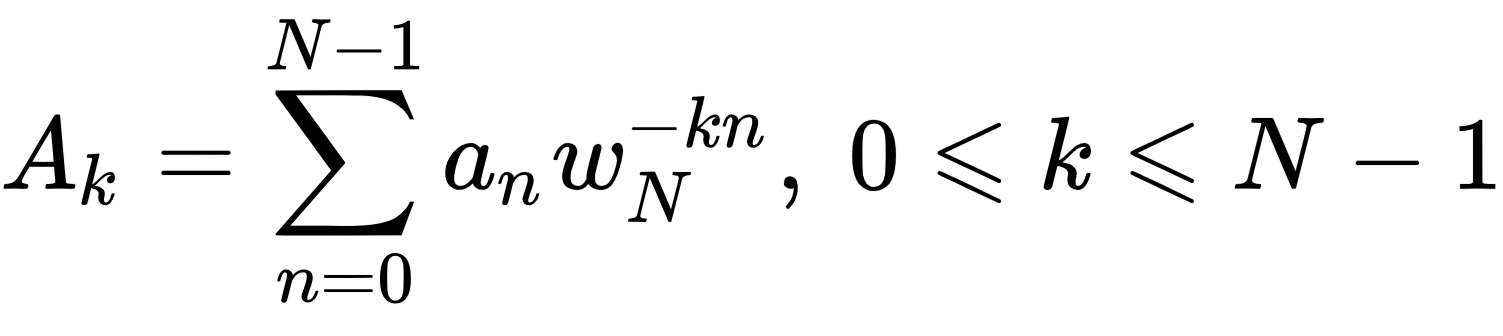
\includegraphics[width=6.3cm]{dft.PNG}
 \vspace{-0.3cm}
 \label{Widok_aplikacjis}
\end{figure}
Odwrotne przekształcenie jest opisane wzorem:
\begin{figure}[h!]
 \centering
 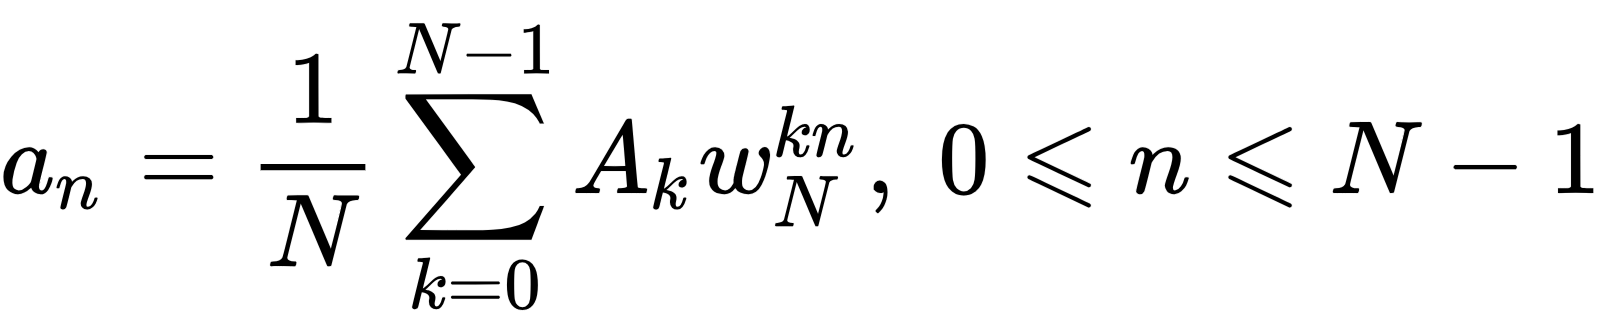
\includegraphics[width=6.3cm]{dftO.PNG}
 \vspace{-0.3cm}
 \label{Splot_indeks}
\end{figure}

x(n) - to wektor próbek sygnału, gdzie kolejne próbki są oddalone od  siebie o czas delta t = 1/fpr (1/częstotliwosć próbkowania).
X(m) -  to wektor-wynik transformacji sygnału x(n). Każda kolejna wartosć opisuje udział składowej częstotliwosci m*f0 w sygnale próbkowanym.
f0 opisuje wzór:
 \\
\begin{figure}[h!]
 \centering
 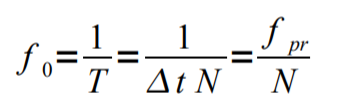
\includegraphics[width=4.3cm]{f0.PNG}
 \vspace{-0.3cm}
 \label{Widok_aplikacjis}
\end{figure}
Istnieje także zapis zastosowaniem jądra transformacji prostej, które przyjmuje postać:
\begin{figure}[h!]
 \centering
 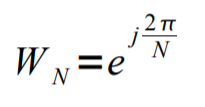
\includegraphics[width=2.3cm]{jadroW.PNG}
 \vspace{-0.3cm}
 \label{Splot_indeks}
\end{figure}
Wtedy zapisujemy:
\newpage
transformacja prosta:
\begin{figure}[h!]
 \centering
 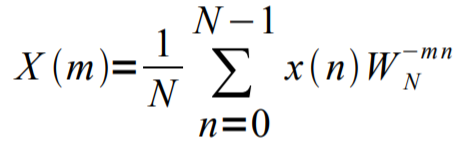
\includegraphics[width=4.8cm]{Xm.PNG}
 \vspace{-0.3cm}
 \label{Splot_indeks}
\end{figure}
\\ transformacja odwrotna:
\begin{figure}[h!]
 \centering
 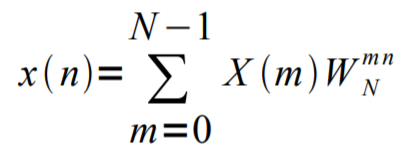
\includegraphics[width=4.3cm]{xn.PNG}
 \vspace{-0.3cm}
 \label{Splot_indeks}
\end{figure}
dla:
\begin{figure}[h!]
 \centering
 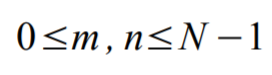
\includegraphics[width=3.3cm]{m,n.PNG}
 \vspace{-0.3cm}
 \label{Splot_indeks}
\end{figure}

Postać macierzowa wzoru przyjmuje postać:
\begin{figure}[h!]
 \centering
 \includegraphics[width=12.3cm]{PMAcierzowa.PNG}
 \vspace{-0.3cm}
 \label{Splot_indeks}
\end{figure}
%%%%%%%%%%%%%%%%%%%%%%%%FFT%%%%%%%%%%%%%%%%%%%%%%%%%%%%%%%%%%%%%%%%%%%%%%%%

\item [Szybka transformacja Fouriera]  - Jest ulepszonym algorytmem DFT z mniejszym kosztem obliczeniowym. Klasyczna Dyskretna transformata Fouriera wymaga N*N mnożeń liczb zespolonych, natomiast FFT N log2 N
\subitem Decymacja w dziedzinie czasu - podział próbek wejściowych, zależnych od czasu, na próbki parzyste i nieparzyste z zapisem do oddziezlbych wektorów.
\\Równanie transformacji, gdy rozdzielimy próbki parzyste i nieparzyste do osobnych wektorów, zapisujemy :

\begin{figure}[h!]
 \centering
 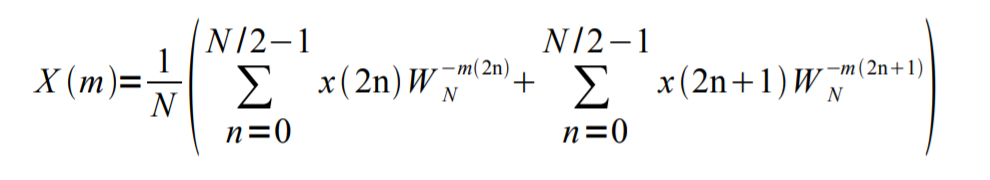
\includegraphics[width=9.3cm]{Decy.PNG}
 \vspace{-0.3cm}
 \label{filtrS}
\end{figure}
\subsubitem f0 = fp/K gdzie f0 to częstotliwosć odcięcia
\subsubitem fp to częstotliwosć 

Po wyciągnięciu WN-m przed sumę, równanie przyjmuje postać:

\begin{figure}[h!]
 \centering
 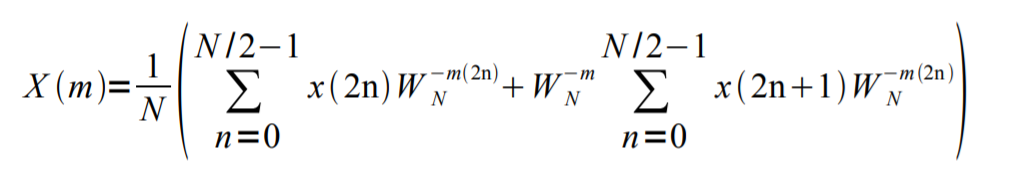
\includegraphics[width=9.3cm]{DecyW.PNG}
 \vspace{-0.3cm}
 \label{filtrS}
\end{figure}

Jedna suma dotyczy próbek parzystych, a drugie nieparzystych.

Ponieważ zachodzi równosć:
\begin{figure}[h!]
 \centering
 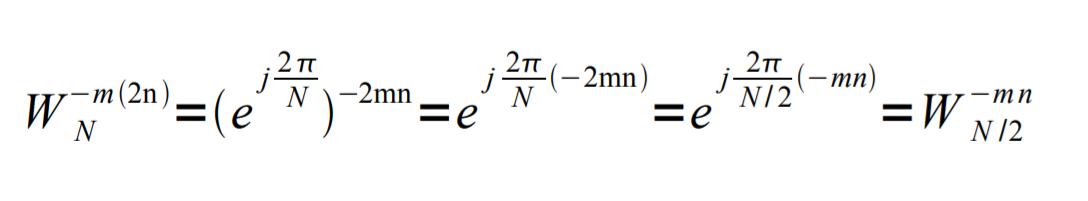
\includegraphics[width=9.3cm]{rownosc.PNG}
 \vspace{-0.3cm}
 \label{filtrS}
\end{figure}
to poprzedni wzór możemy zapisać jako:
\begin{figure}[h!]
 \centering
 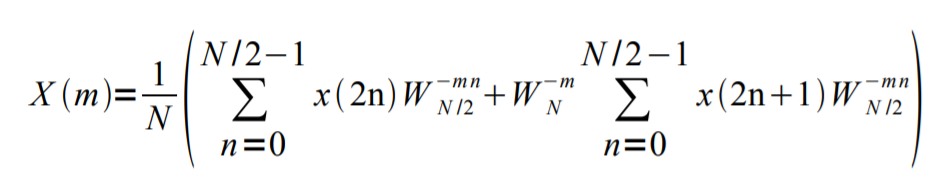
\includegraphics[width=9.3cm]{FFTr.PNG}
 \vspace{-0.3cm}
 \label{filtrS}
\end{figure}

Sumowane wyrażenia są analogiczne do  postaci wejciowej ale dotyczą tylko połowy próbek. Współczynnik m ma wartosć od 0 do N-1.
Mamy:
\begin{figure}[h!]
 \centering
 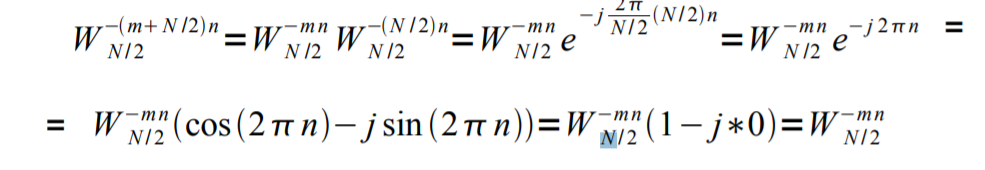
\includegraphics[width=12.3cm]{mamy.PNG}
 \vspace{-0.3cm}
 \label{sp}
\end{figure}
co oanqcza, że drugą połową wektora jest powtórzenie pierwszej połowy. Pozwala to na wykonanie N/2 sumowań zamiast N. Stosując te same operacje dla N - nieparzystych. Teraz są mnożone maciezrzy to N/2xN/2 zamiast NxN. Trzeba jeszcze pomnożyć N razy przy składaniu wektorów, ale koszt nadal jest dużo mniejszy.
\\ Jako metodę obliczania FFT można zastosować algorytm motylkowy:
\begin{figure}[h!]
 \centering
 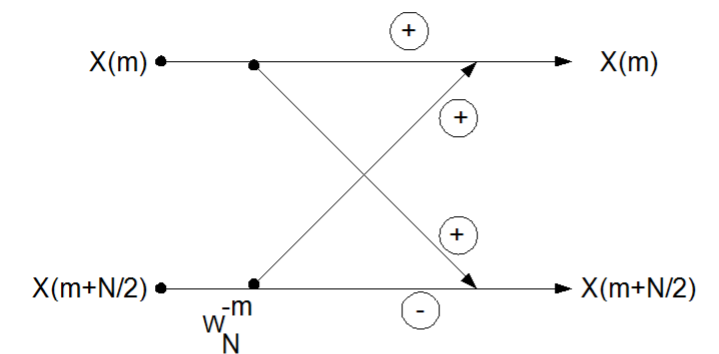
\includegraphics[width=9.3cm]{motylek.PNG}
 \vspace{-0.3cm}
 \label{sp}
\end{figure}
W motylku wartość X(m+N/2) mnoży się przez odpowiedni współczynnik WN-m odczytany z wektora. Wyniki z prawej strony są uzyskiwane jako suma wartości ze strony lewej (X(m)) oraz jako różnica tych wartości (X(m+N/2)). Znak minus wynika z faktu, że w drugiej połowie wektora współczynników są wartości przeciwne do tych z pierwszej.  


%%%%%%%%%%%%%%%%%%%%%%%%TRANSFORMACJA KOSINUSOWA%%%%%%%%%%%%%%%%%%%%%%%%%%%%%%%%%%%%%

\item [Transformacja kosinusowa] - wykorzystanie funkcji cosinus o różnych fazach i okresach. DCT II opisuje wzór:
\begin{figure}[h!]
 \centering
 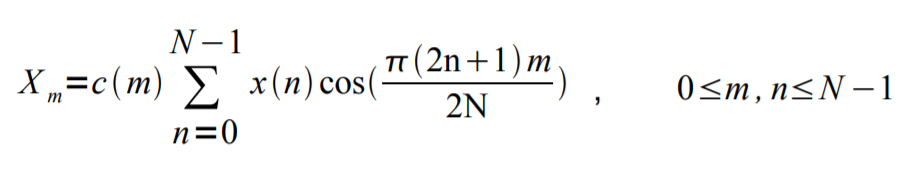
\includegraphics[width=9.3cm]{DCT2.PNG}
 \vspace{-0.3cm}
 \label{kr}
\end{figure}
\\ a przekształcenie odwrotne przyjmuje postać: 
\begin{figure}[h!]
 \centering
 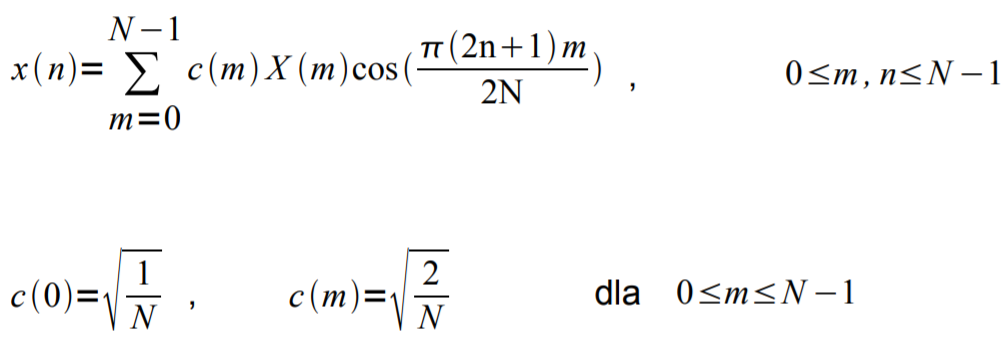
\includegraphics[width=10.3cm]{DCT2O.PNG}
 \vspace{-0.3cm}
 \label{kw}
\end{figure}

Sygnał y(n) to sygnał x(n) o zmienionej kolejności próbek, gdzie w pierwszej połowie znajdują się próbki parzyste, a w drugiej próbki nieparzyste w odwróconej kolejnosci.



%%%%%%%%%%%%%%%%%%%%%%%%SZYBKA TRANSFORMACJA KOSINUSOWA%%%%%%%%%%%%%%%%%%%%%%%%%%%%%%%%%%%%%

\item [Szybka transformacja kosinusowa] - zastosowanie szybkich algorytmów dyskretnej transformacji Fouriera, stosowanych przy przekształceniu
równania DCT do postaci pozwalającej wyodrębnić z niego człon stanowiący DFT. 
\\ Gdy mamy sygnał dyskretny opisany jako funkcja można zdefiniować
sygnał y(n) wzorami:
\begin{figure}[h!]
 \centering
 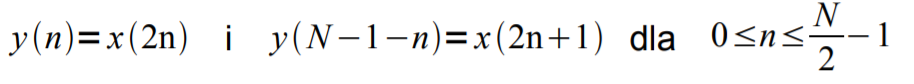
\includegraphics[width=8.3cm]{yn.PNG}
 \vspace{-0.3cm}
 \label{kr}
\end{figure}
\\ a przekształcenie odwrotne przyjmuje postać: 
\newpage
\begin{figure}[h!]
 \centering
 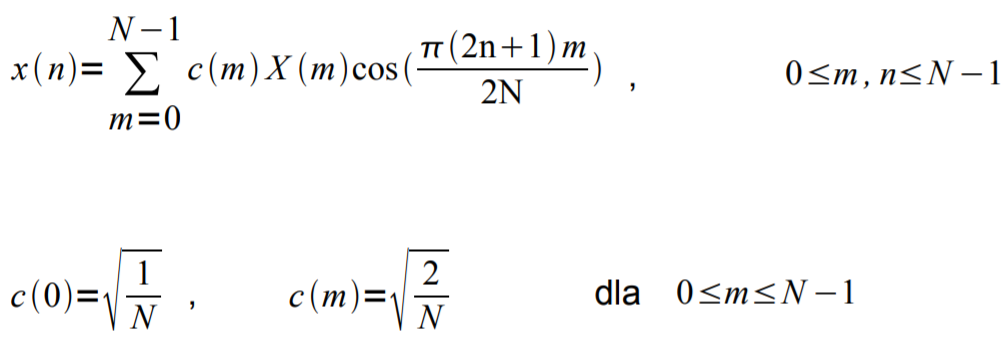
\includegraphics[width=9.3cm]{DCT2O.PNG}
 \vspace{-0.3cm}
 \label{kw}
\end{figure}

Transformatę sygnału x(n) można obliczyćprzy pomocy wzoru:
\begin{figure}[h!]
 \centering
 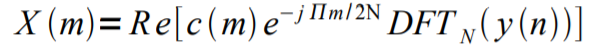
\includegraphics[width=6.3cm]{xmF.PNG}
 \vspace{-0.3cm}
 \label{kw}
\end{figure}
Przy czym przekształcenie odwrotne opisuje rówananie:
\begin{figure}[h!]
 \centering
 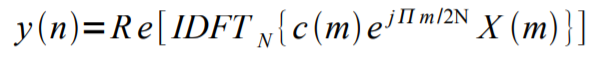
\includegraphics[width=6.3cm]{xmFO.PNG}
 \vspace{-0.3cm}
 \label{kw}
\end{figure}

Sygnał x(n) odtwarzamy przy pomocy zmiany kolejności próbek w sygnale y(n).

\end{labeling}

%%%%%%%%%%%%%%%%%%%%%%%%INSTRUKCA OBSŁUGI%%%%%%%%%%%%%%%%%%%%%%%%%%%%%%%%%%%%%%%%%%%%

\subsection{Instrukcja obsługi aplikacji}
Aplikacja do generacji szumów zawiera interfejs graficzny, który służy do obsługi przez użytkownika. Wygląd został przedstawiony na poniższym rysunku.
\begin{figure}[h!]
 \centering
 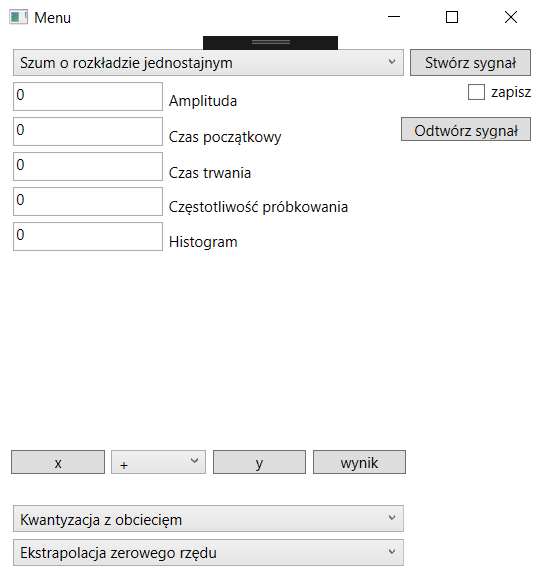
\includegraphics[width=6.3cm]{ui1.PNG}
 \vspace{-0.3cm}
 \caption{Widok główny aplikacji}
 \label{Widok_aplikacjis}
\end{figure}

Na górze okienka znajduje się wysuwana lista możliwych do generacji sygnałów. Obok znajduje się chceckbox, po zaznaczeniu którego sygnał zostanie zapisany do pliku.
Niżej jest przycisk do generacji sygnałów oraz lista parametrów wykresu. Tutaj wpisuje się dane wpływające na sygnał.
Pola umożliwiają ustawienie charakterystycznych parametrów sygnału. Na ich podstawie program wylicza wartości amplitudy sygnału w określonym czasie oraz wyświetla graficzną reprezentację sygnału w postaci wykresu funkcji amplitudy od czasu i histogramu.\\

Na dole okienka znajdują się przyciski do operacji na dwóch sygnałach (dodawanie, odejmowanie itp, a także splot, korelacja). Po kliknięciu w x i y wybieramy odpowiednio pierwszy i dugi składnik działania. Po wcisnięciu przycisku "wynik" program liczy wynik działania i wywietla jego graficzną reprezentację. 
Poniżej znajdują się wysuwane listy z opcjami kwantyzacji, ekstrapolacji. Niżej znajdują się okienka służące do wpisywania parametróW filtracji. Pod nimi znajdują się do wyboru warianty okna i filtru.
Na samym dole okna jest okienko do wpisywania parametrów radaru. 

\subsubsection{Generowanie sygnału}
Aby wygenerować sygnał użytkownik musi kliknąć w generuj sygnał lub w przypadku innych operacji wynik.
\\Po wygenerowaniu sygnału pojawiają się dodatkowe okienko aplikacji.
\begin{figure}[h!]
 \centering
 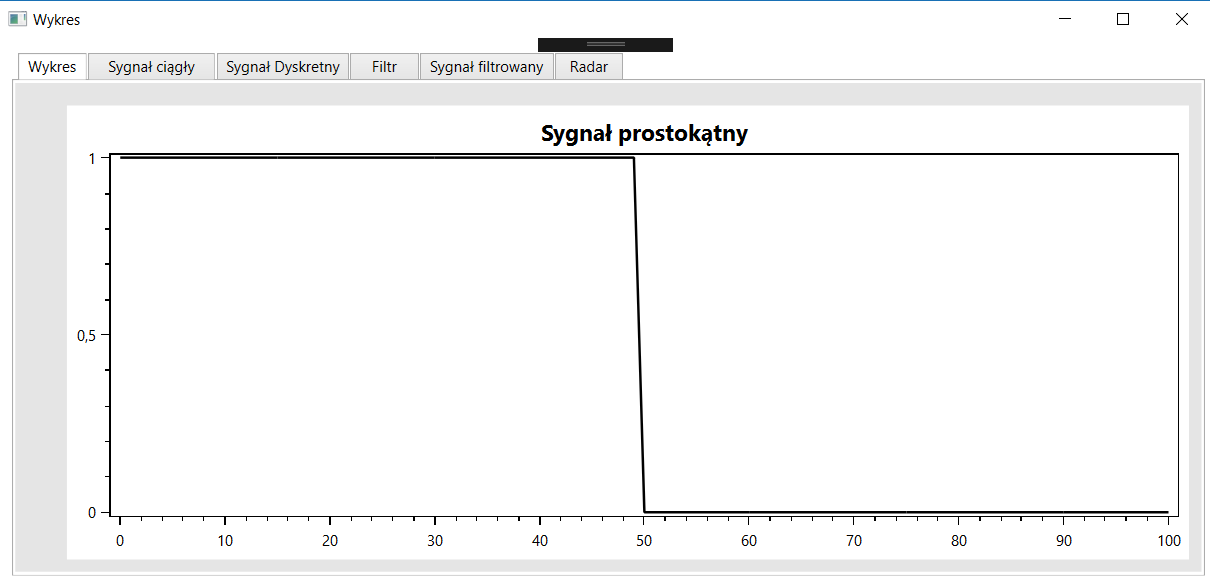
\includegraphics[width=15.3cm]{prost.PNG}
 \vspace{-0.3cm}
 \caption{Okna po generacji sygnału}
 \label{Widok_aplikacjis}
\end{figure}
\\W kolejnych zakładkach okienka są inne wykresy.

\subsubsection{Odczyt sygnału z pliku}
Oprócz generacji i zapisu do pliku, program umożliwia odczyt z pliku sygnału będącego wynikiem dyskretyzacji (bez kwantyzacji) wygenerowanego
sygnału ciągłego oraz sygnału będącego wynikiem operacji na dwóch sygnałach dyskretnych.
\\Tak jak w przypadku generacji, sygnał jest  reprezentowany graficznie w postaci histogramu i wykresu funkcji.

\subsection{Opis implementacji}
Aplikacja została napisana w wysokopoziomowym języku programowania - C\#. Do rysowania wykresów została wykorzystana zewnątrzna biblioteka OxyPlot. Program został napisany przy pomocy metodyki obiektowej i stosuje metody numeryczne.

\section{Eksperymenty i wyniki}

Poniżej znajdują się wszystkie przeprowadzone eksperymenty - możliwe do uzyskania w aplikacji sygnaly i wyniki. 

%%%%%%%%%%%%%%%%%%%%%%%%%%%%%%%%%%%%%%%%%%%%%%%%%%%%%%%%%%%%%%%%%%%%%%%%%%%%%%%%%%%%%%%%%%%%%%%%%%%%%%%%%%%%%%%%%
% PODROZDZIA PT. EKSPERYMENT NR 1 
%%%%%%%%%%%%%%%%%%%%%%%%%%%%%%%%%%%%%%%%%%%%%%%%%%%%%%%%%%%%%%%%%%%%%%%%%%%%%%%%%%%%%%%%%%%%%%%%%%%%%%%%%%%%%%%%%

\subsection{Eksperyment nr 1}

Eksperyment nr 1 -  DFT\\


\subsubsection{Założenia}
Program wykona obliczenia niezbędne do obliczenia dyskretnej transformaty Fouriera \ref{Splot_indeks}.

\subsubsection{Przebieg}
Do generacji synału zostały podane parametry:
\addtokomafont{labelinglabel}{\sffamily}

\begin{labeling}{szj}
\item [Sygnał 1:] 
\subitem [ n:] 3
\begin{figure}[h!]
 \centering
 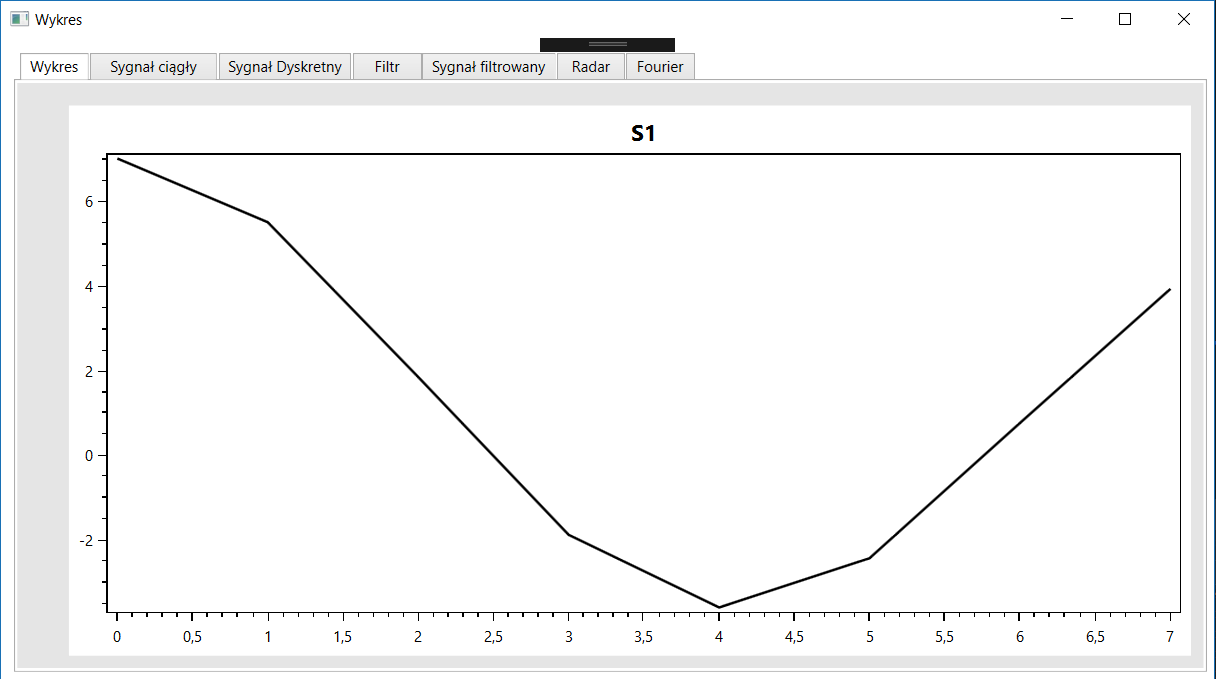
\includegraphics[width=12.3cm]{s13.PNG}
 \vspace{-0.3cm}
 \caption{Wykres funkcji}
 \label{sin}
\end{figure}

\item [Sygnał 2:] 
\subitem [ n:] 6
\begin{figure}[h!]
 \centering
 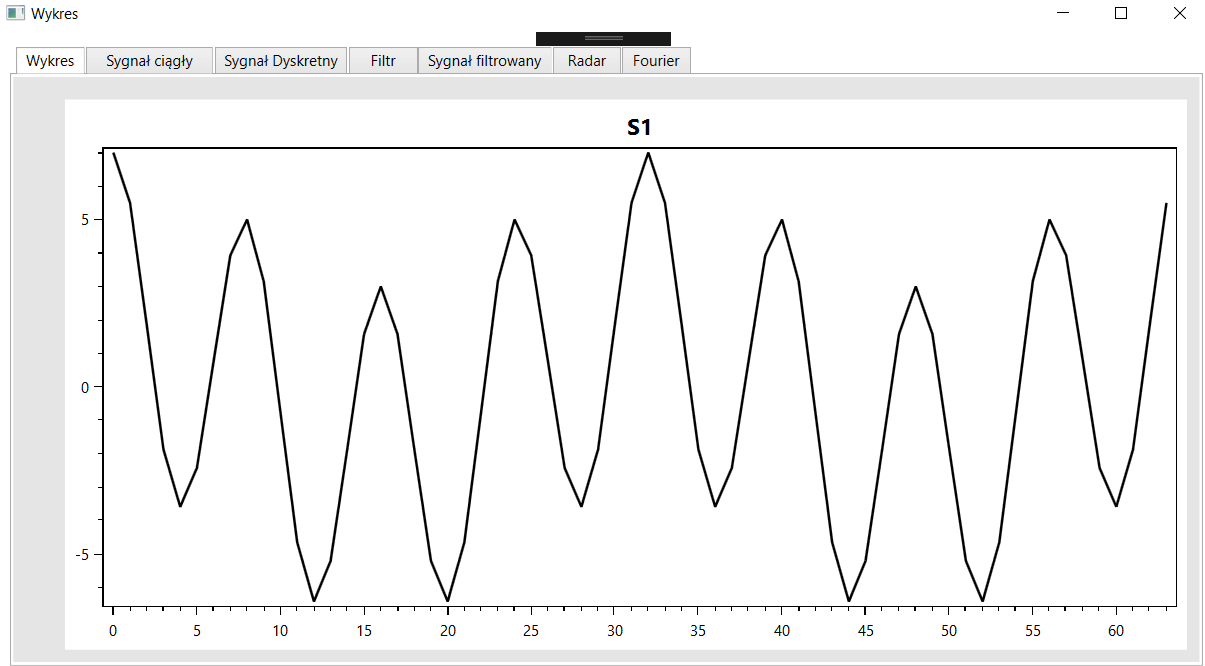
\includegraphics[width=12.3cm]{s16.PNG}
 \vspace{-0.3cm}
 \caption{Wykres funkcji}
 \label{sin}
\end{figure}

\item [Sygnał 3:] 
\subitem [ n:] 8
\begin{figure}[h!]
 \centering
 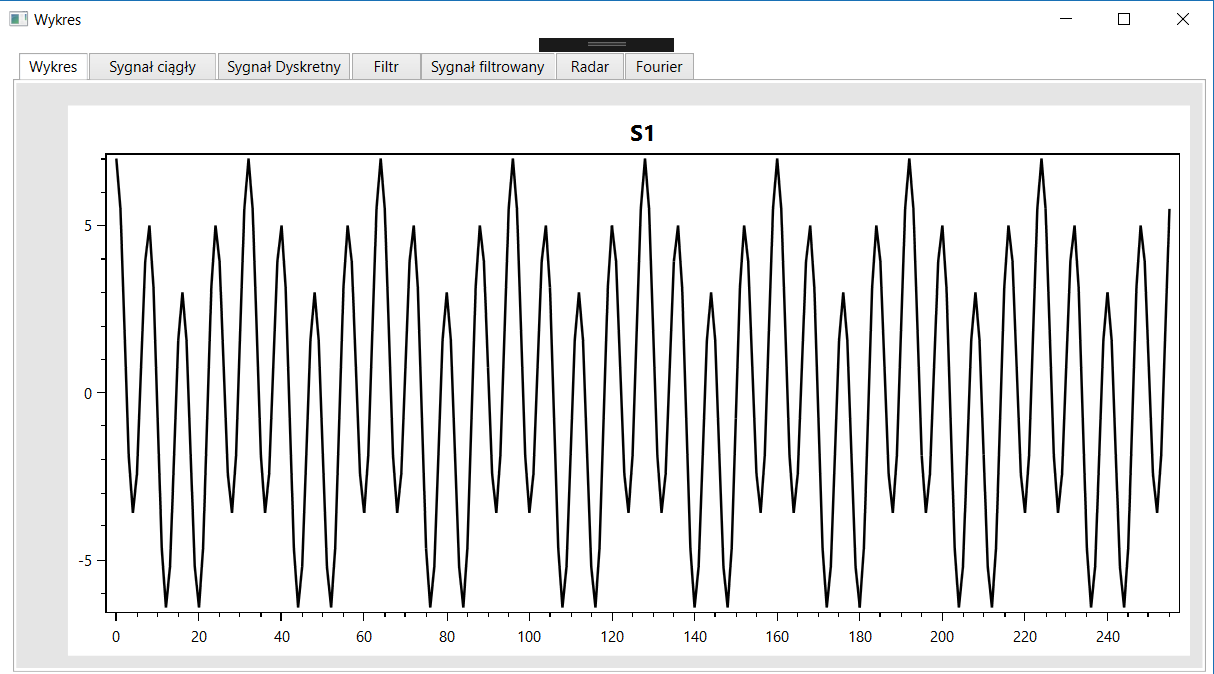
\includegraphics[width=12.3cm]{s18.PNG}
 \vspace{-0.3cm}
 \caption{Wykres funkcji}
 \label{sin}
\end{figure}


\end{labeling}

\subsubsection{Rezultat}

Rezultaty przedstawiają zamieszczone poniżej zrzut ekranu z programu. Czas wykonania oraz wykres dyskretnej transformaty Fouriera.

 Sygnał 1:
\begin{figure}[h!]
 \centering
 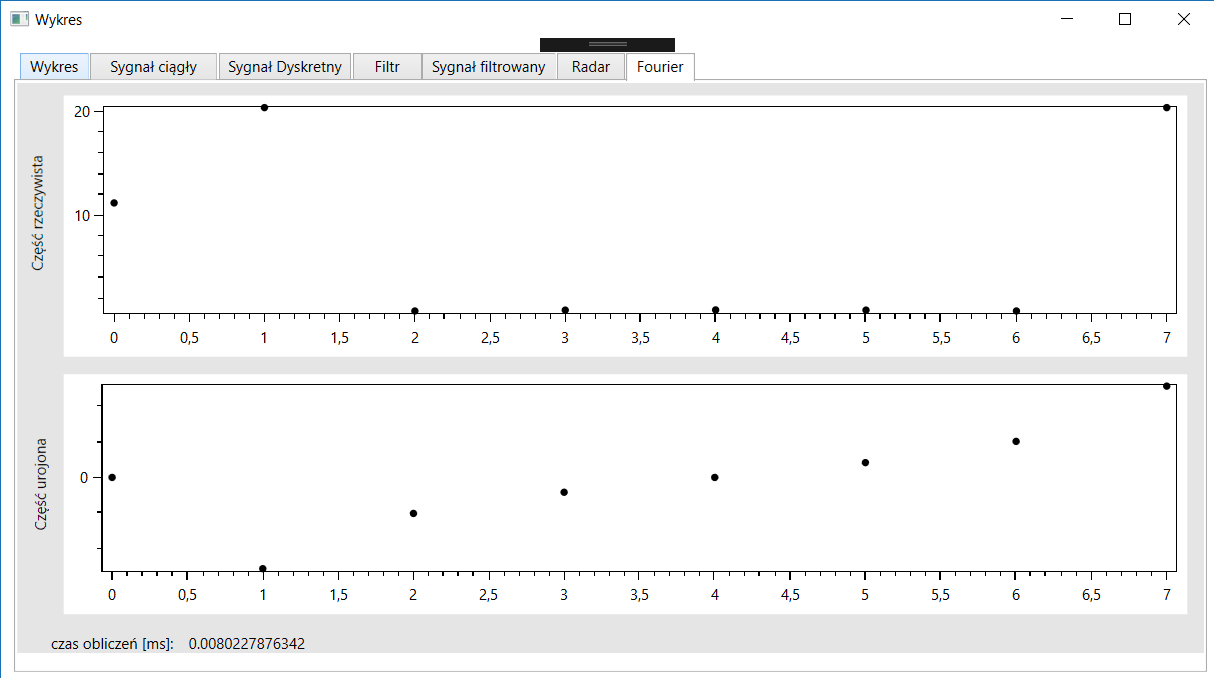
\includegraphics[width=12.3cm]{s13F.PNG}
 \vspace{-0.3cm}
 \caption{Wykres DFT dla sygnału 1}
 \label{Wykres dla wynikw eksperymentu pierwszego}
\end{figure}

Sygnał 2:
\begin{figure}[h!]
 \centering
 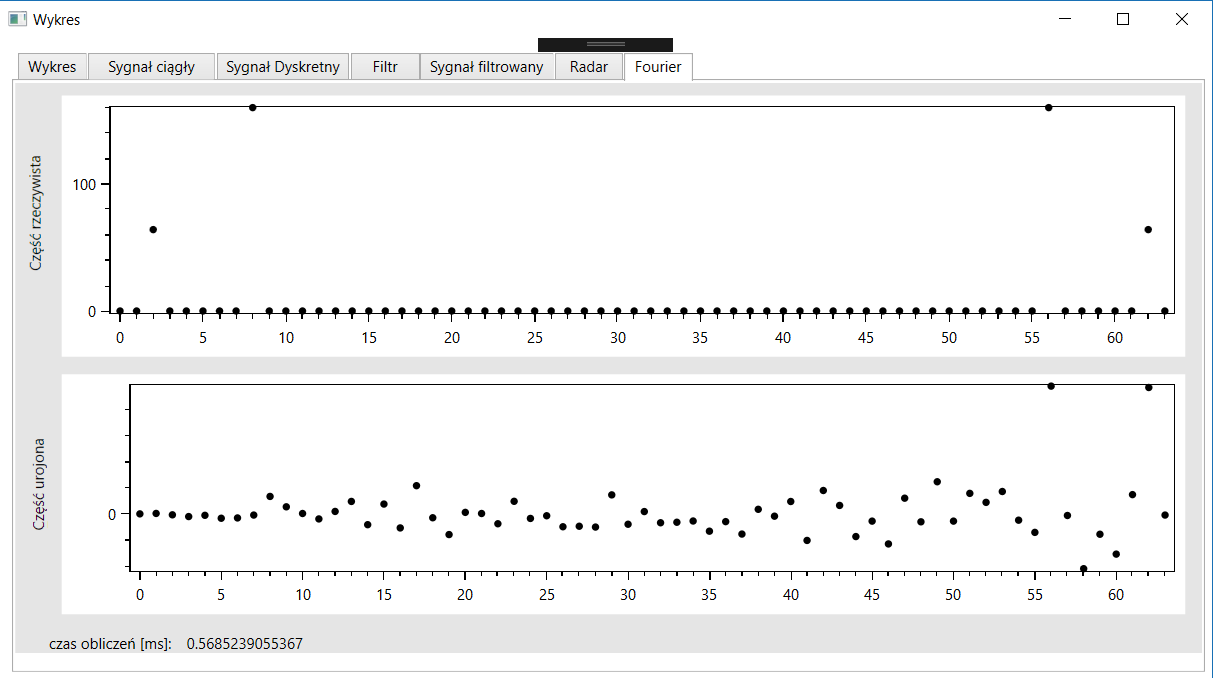
\includegraphics[width=12.3cm]{s16F.PNG}
 \vspace{-0.3cm}
 \caption{Wykres DFT dla sygnału 2}
 \label{Wykres dla wynikw eksperymentu pierwszego}
\end{figure}

\newpage
Sygnał 3:
\begin{figure}[h!]
 \centering
 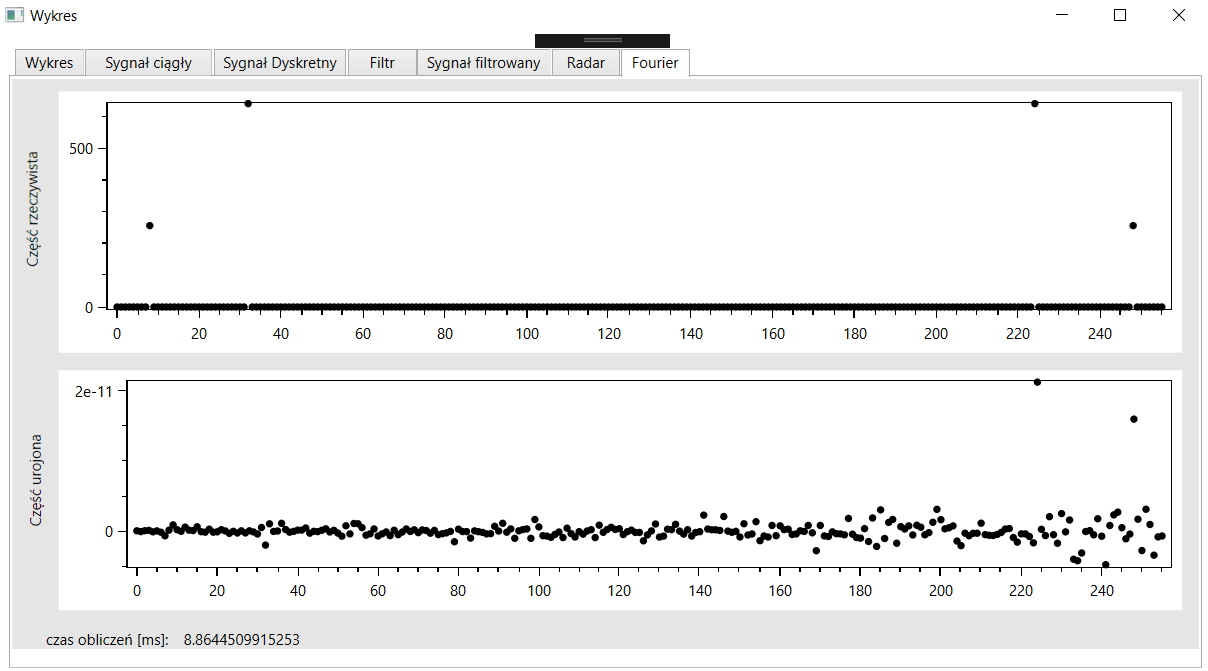
\includegraphics[width=12.3cm]{s18F.PNG}
 \vspace{-0.3cm}
 \caption{Wykres DFT dla sygnału 3}
 \label{Wykres dla wynikw eksperymentu pierwszego}
\end{figure}

%%%%%%%%%%%%%%%%%%%%%%%%%%%%%%%%%%%%%%%%%%%%%%%%%%%%%%%%%%%%%%%%%%%%%%%%%%%%%%%%%%%%%%%%%%%%%%%%%%%%%%%%%%%%%%%%%
% PODROZDZIA PT. EKSPERYMENT NR2 
%%%%%%%%%%%%%%%%%%%%%%%%%%%%%%%%%%%%%%%%%%%%%%%%%%%%%%%%%%%%%%%%%%%%%%%%%%%%%%%%%%%%%%%%%%%%%%%%%%%%%%%%%%%%%%%%%

\subsection{Eksperyment nr 2}
Eksperyment nr 2  - FFT
\subsubsection{Założenia}
Program wykona obliczenia niezbędne do obliczenia dyskretnej transformaty Fouriera \ref{Splot_indeks}.

\subsubsection{Przebieg}
Do generacji synału zostały podane parametry:
\addtokomafont{labelinglabel}{\sffamily}

\begin{labeling}{szj}

\item [Sygnał 1:] 
\subitem [ n:] 3
\begin{figure}[h!]
 \centering
 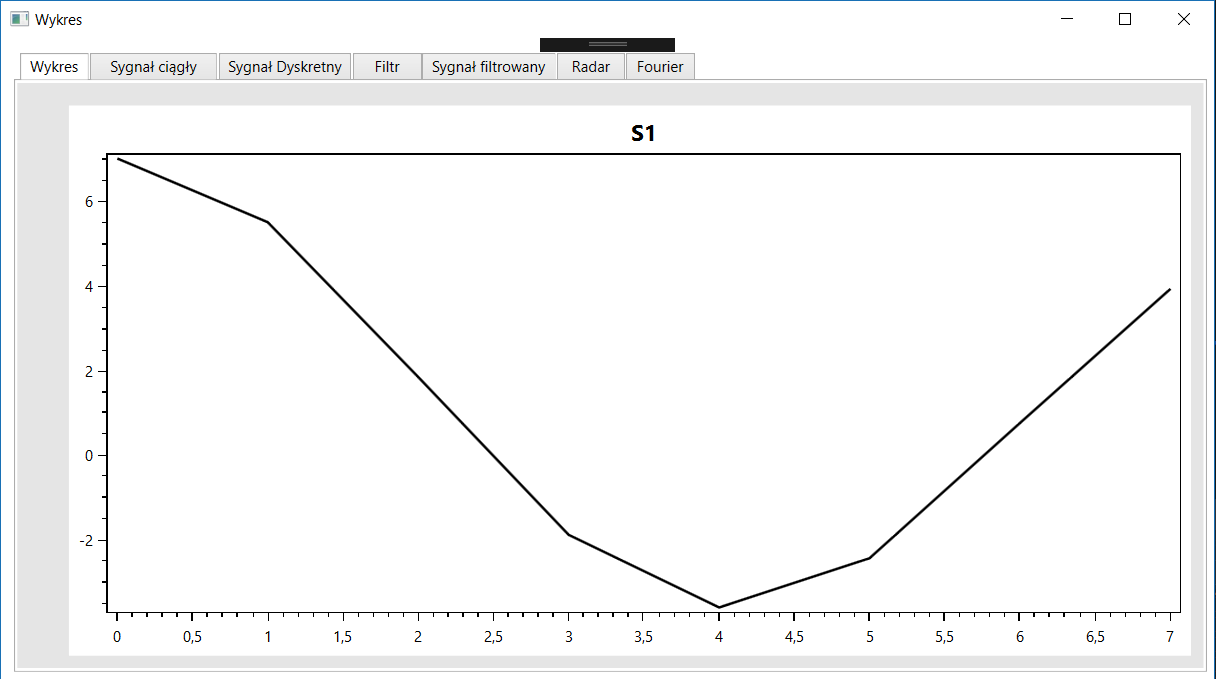
\includegraphics[width=12.3cm]{s13.PNG}
 \vspace{-0.3cm}
 \caption{Wykres funkcji}
 \label{sin}
\end{figure}

\newpage
\item [Sygnał 2:] 
\subitem [ n:] 6
\begin{figure}[h!]
 \centering
 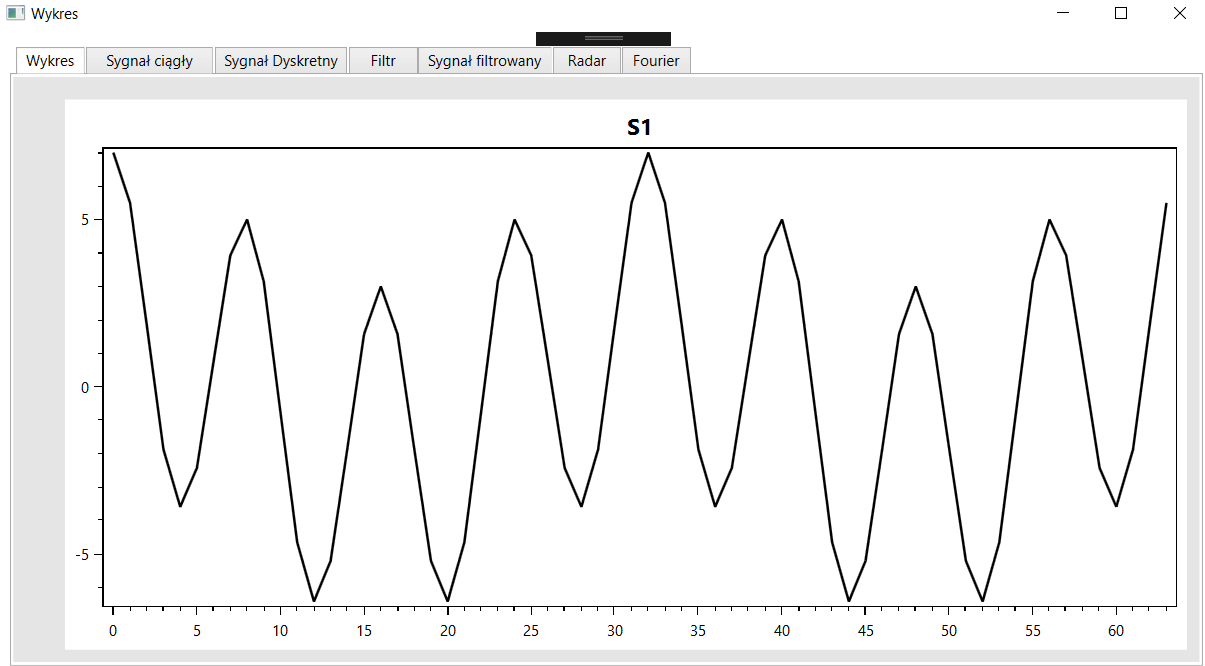
\includegraphics[width=12.3cm]{s16.PNG}
 \vspace{-0.3cm}
 \caption{Wykres funkcji}
 \label{sin}
\end{figure}

\item [Sygnał 3:] 
\subitem [ n:] 8
\begin{figure}[h!]
 \centering
 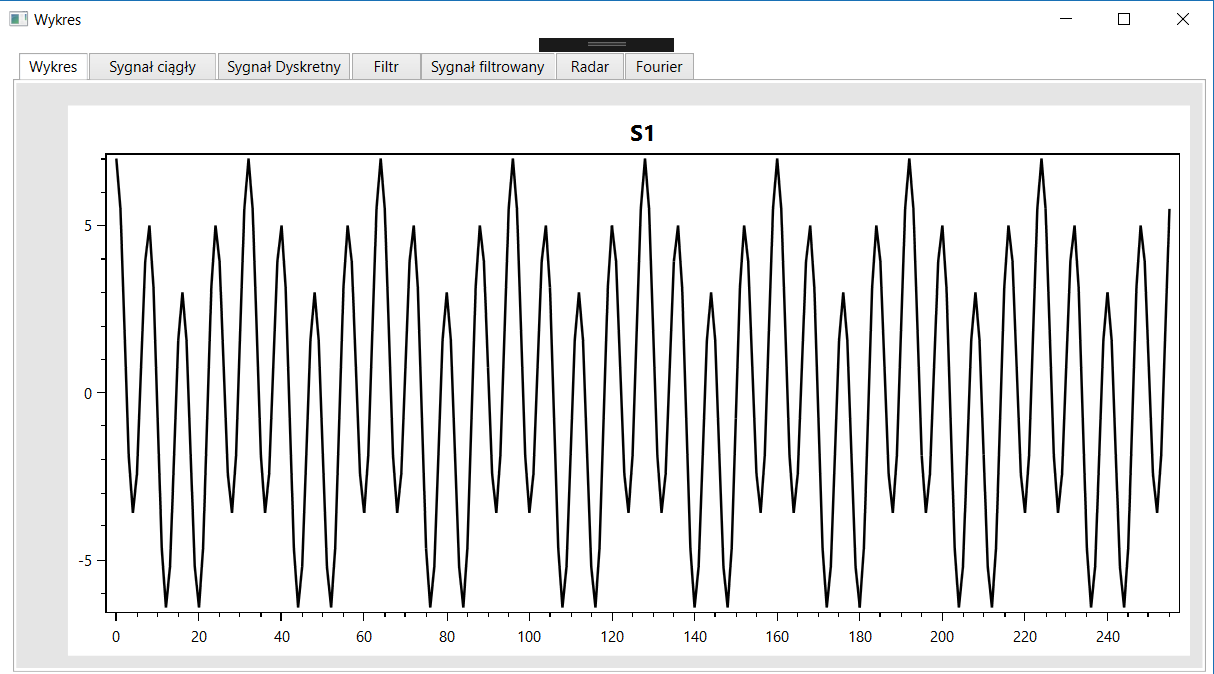
\includegraphics[width=12.3cm]{s18.PNG}
 \vspace{-0.3cm}
 \caption{Wykres funkcji}
 \label{sin}
\end{figure}


\end{labeling}

\subsubsection{Rezultat}

Rezultaty przedstawiają zamieszczone poniżej zrzut ekranu z programu. Czas wykonania oraz wykres dyskretnej transformaty Fouriera.
\newpage
 Sygnał 1:
\begin{figure}[h!]
 \centering
 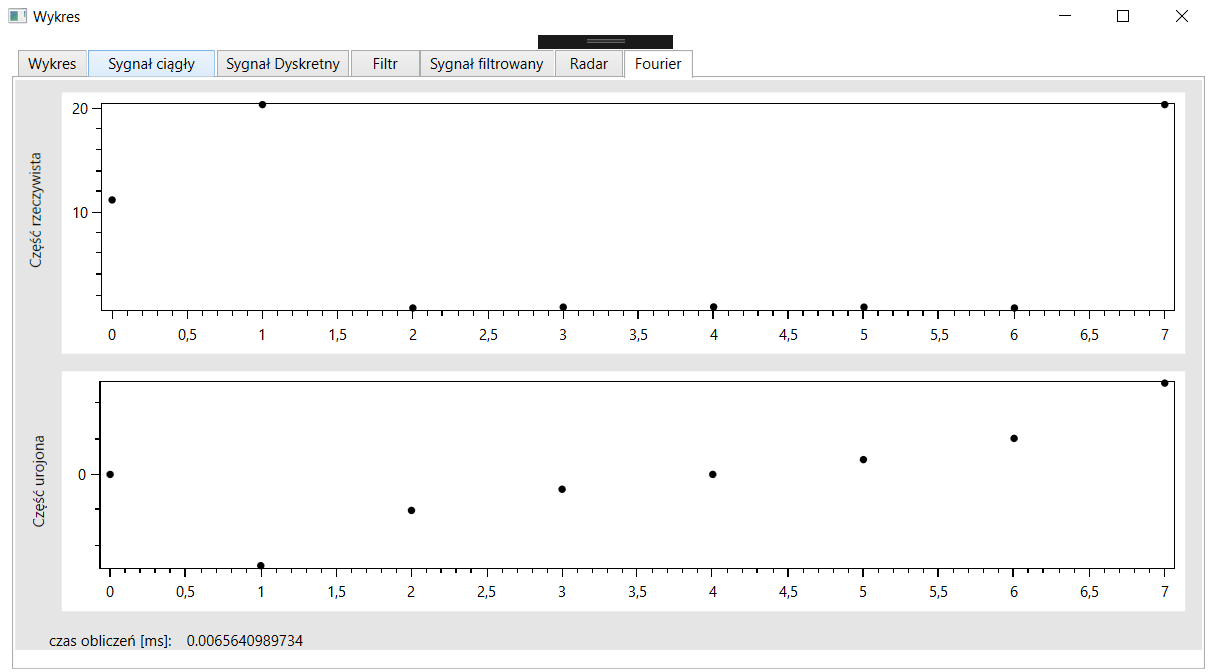
\includegraphics[width=12.3cm]{s13FFT.PNG}
 \vspace{-0.3cm}
 \caption{Wykres FFT dla sygnału 1}
 \label{Wykres dla wynikw eksperymentu pierwszego}
\end{figure}

Sygnał 2:
\begin{figure}[h!]
 \centering
 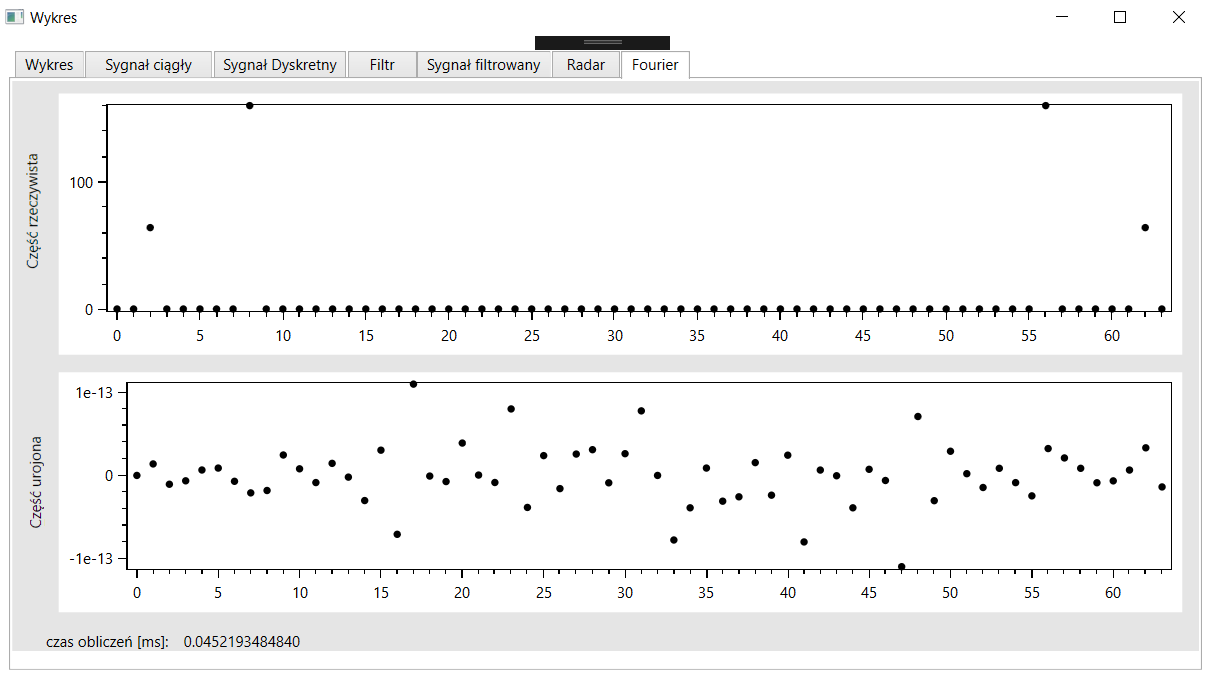
\includegraphics[width=12.3cm]{s16FFT.PNG}
 \vspace{-0.3cm}
 \caption{Wykres FFT dla sygnału 2}
 \label{Wykres dla wynikw eksperymentu pierwszego}
\end{figure}

\newpage
Sygnał 3:
\begin{figure}[h!]
 \centering
 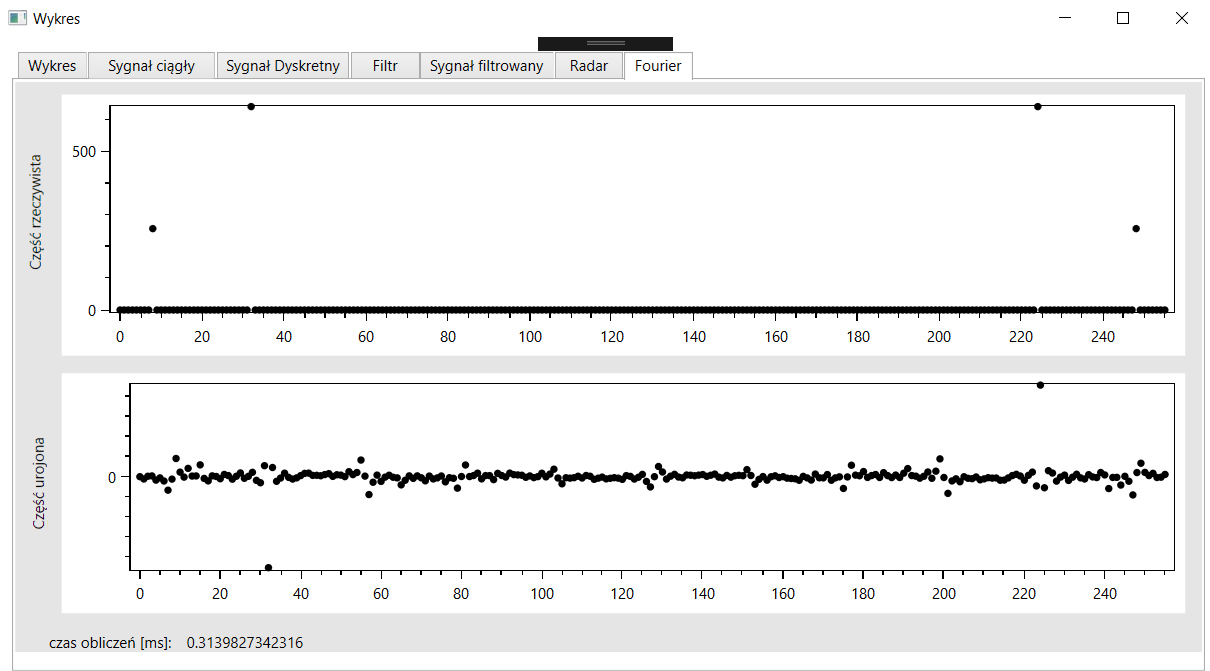
\includegraphics[width=12.3cm]{s18FFT.PNG}
 \vspace{-0.3cm}
 \caption{Wykres FFT dla sygnału 3}
 \label{Wykres dla wynikw eksperymentu pierwszego}
\end{figure}

%%%%%%%%%%%%%%%%%%%%%%%%%%%%%%%%%%%%%%%%%%%%%%%%%%%%%%%%%%%%%%%%%%%%%%%%%%%%%%%%%%%%%%%%%%%%%%%%%%%%%%%%%%%%%%%%%
% PODROZDZIA PT. EKSPERYMENT NR 3
%%%%%%%%%%%%%%%%%%%%%%%%%%%%%%%%%%%%%%%%%%%%%%%%%%%%%%%%%%%%%%%%%%%%%%%%%%%%%%%%%%%%%%%%%%%%%%%%%%%%%%%%%%%%%%%%%

\subsection{Eksperyment nr 3}

Eksperyment nr 3  -transformacja kosinusowa typu drugiego 
\subsubsection{Założenia}
Program wykonuje transformację kosinusową typu drugiego

\subsubsection{Przebieg}
Do generacji synału zostały podane parametry:
\addtokomafont{labelinglabel}{\sffamily}

\begin{labeling}{szj}
\newpage
\item [Sygnał 1:] 
\subitem [ n:] 3
\begin{figure}[h!]
 \centering
 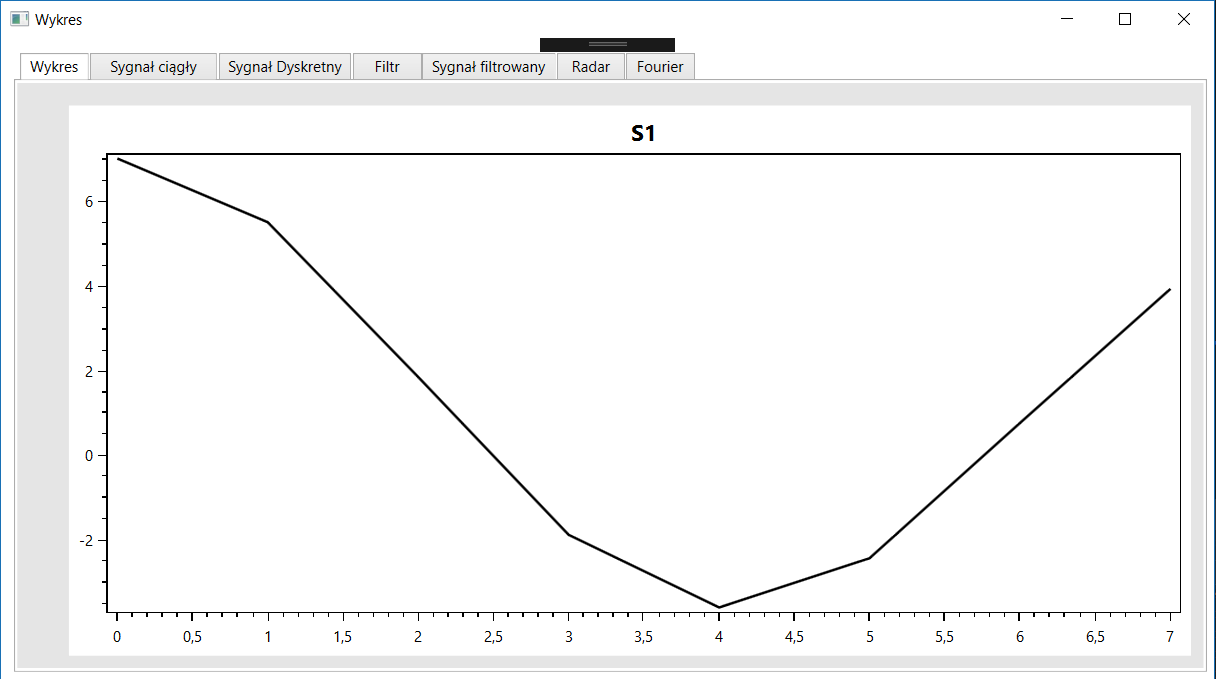
\includegraphics[width=12.3cm]{s13.PNG}
 \vspace{-0.3cm}
 \caption{Wykres funkcji}
 \label{sin}
\end{figure}

\item [Sygnał 2:] 
\subitem [ n:] 6
\begin{figure}[h!]
 \centering
 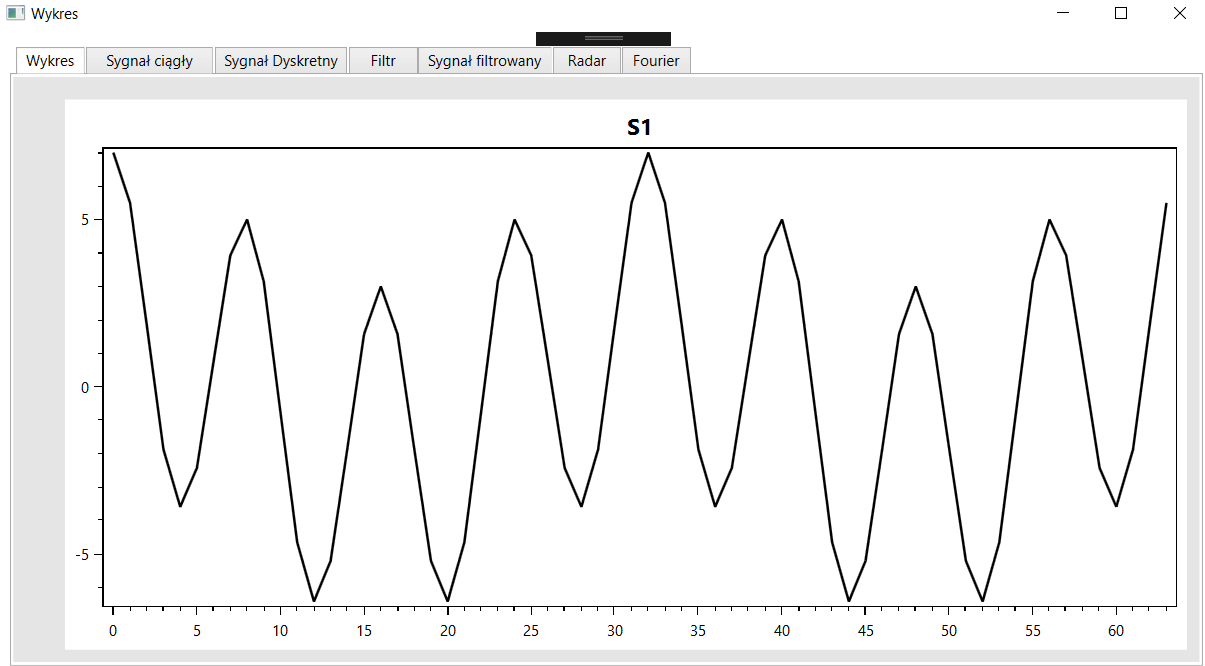
\includegraphics[width=12.3cm]{s16.PNG}
 \vspace{-0.3cm}
 \caption{Wykres funkcji}
 \label{sin}
\end{figure}

\item [Sygnał 3:] 
\subitem [ n:] 8
\begin{figure}[h!]
 \centering
 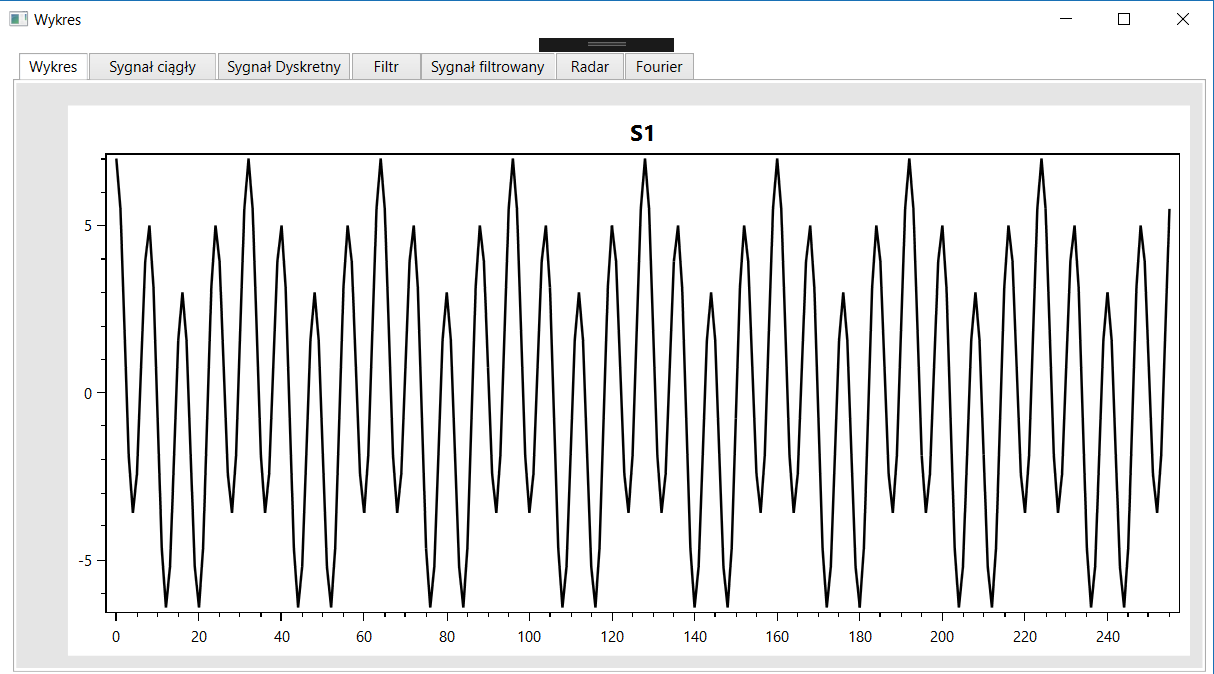
\includegraphics[width=12.3cm]{s18.PNG}
 \vspace{-0.3cm}
 \caption{Wykres funkcji}
 \label{sin}
\end{figure}


\end{labeling}

\subsubsection{Rezultat}

Rezultaty przedstawiają zamieszczone poniżej zrzut ekranu z programu. Czas wykonania oraz wykres transformaciji kosinusowej typu drugiego
\newpage
 Sygnał 1:
\begin{figure}[h!]
 \centering
 \includegraphics[width=12.3cm]{s13DCT2.PNG}
 \vspace{-0.3cm}
 \caption{Wykres DCT II dla sygnału 1}
 \label{Wykres dla wynikw eksperymentu pierwszego}
\end{figure}

Sygnał 2:
\begin{figure}[h!]
 \centering
 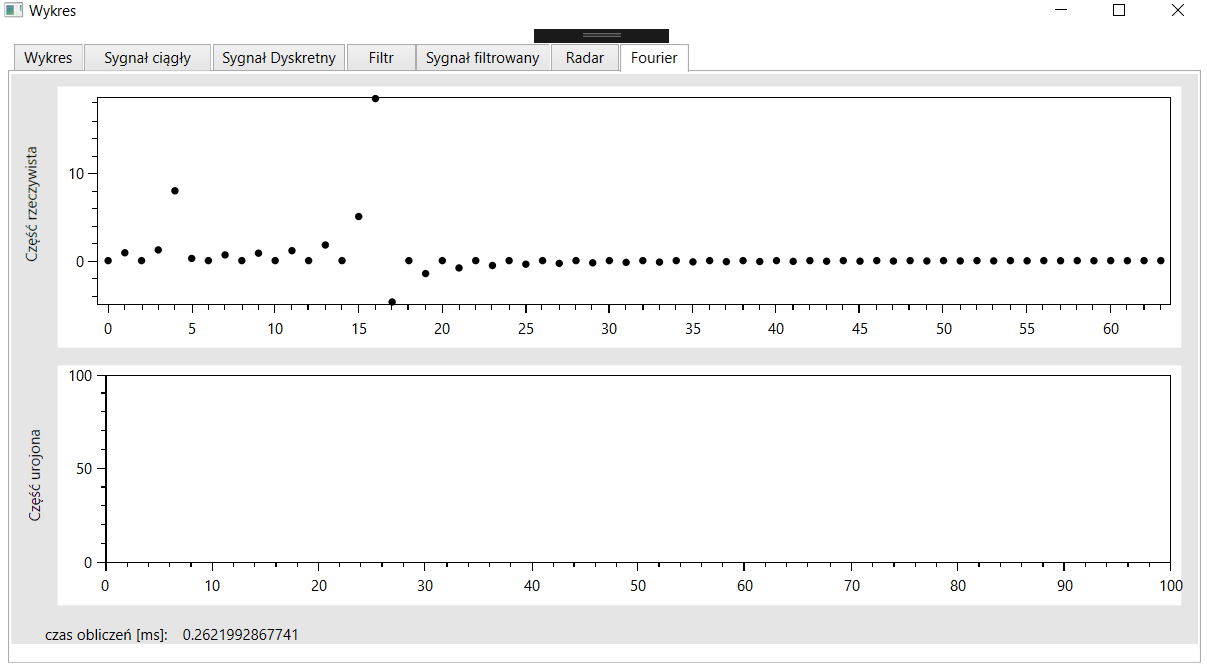
\includegraphics[width=12.3cm]{s16DCT2.PNG}
 \vspace{-0.3cm}
 \caption{Wykres DCT II dla sygnału 2}
 \label{Wykres dla wynikw eksperymentu pierwszego}
\end{figure}

\newpage
Sygnał 3:
\begin{figure}[h!]
 \centering
 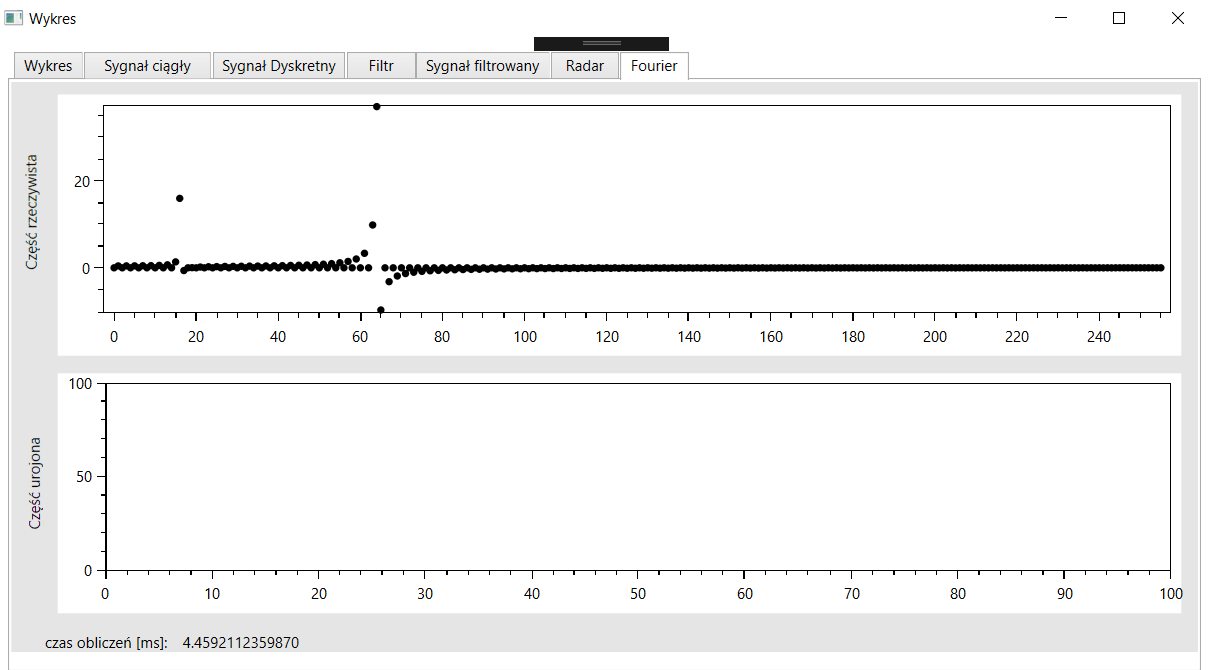
\includegraphics[width=12.3cm]{s18DCT2.PNG}
 \vspace{-0.3cm}
 \caption{Wykres DCT II dla sygnału 3}
 \label{Wykres dla wynikw eksperymentu pierwszego}
\end{figure}

%%%%%%%%%%%%%%%%%%%%%%%%%%%%%%%%%%%%%%%%%%%%%%%%%%%%%%%%%%%%%%%%%%%%%%%%%%%%%%%%%%%%%%%%%%%%%%%%%%%%%%%%%%%%%%%%%
% PODROZDZIA PT. EKSPERYMENT NR 4 
%%%%%%%%%%%%%%%%%%%%%%%%%%%%%%%%%%%%%%%%%%%%%%%%%%%%%%%%%%%%%%%%%%%%%%%%%%%%%%%%%%%%%%%%%%%%%%%%%%%%%%%%%%%%%%%%%

\subsection{Eksperyment nr 4}

Eksperyment nr 4  - Szybka transformacja kosinusowa
\subsubsection{Założenia}
Program wykonuje transformację kosinusową typu drugiego

\subsubsection{Przebieg}
Do generacji synału zostały podane parametry:
\addtokomafont{labelinglabel}{\sffamily}

\begin{labeling}{szj}

\item [Sygnał 1:] 
\subitem [ n:] 3
\begin{figure}[h!]
 \centering
 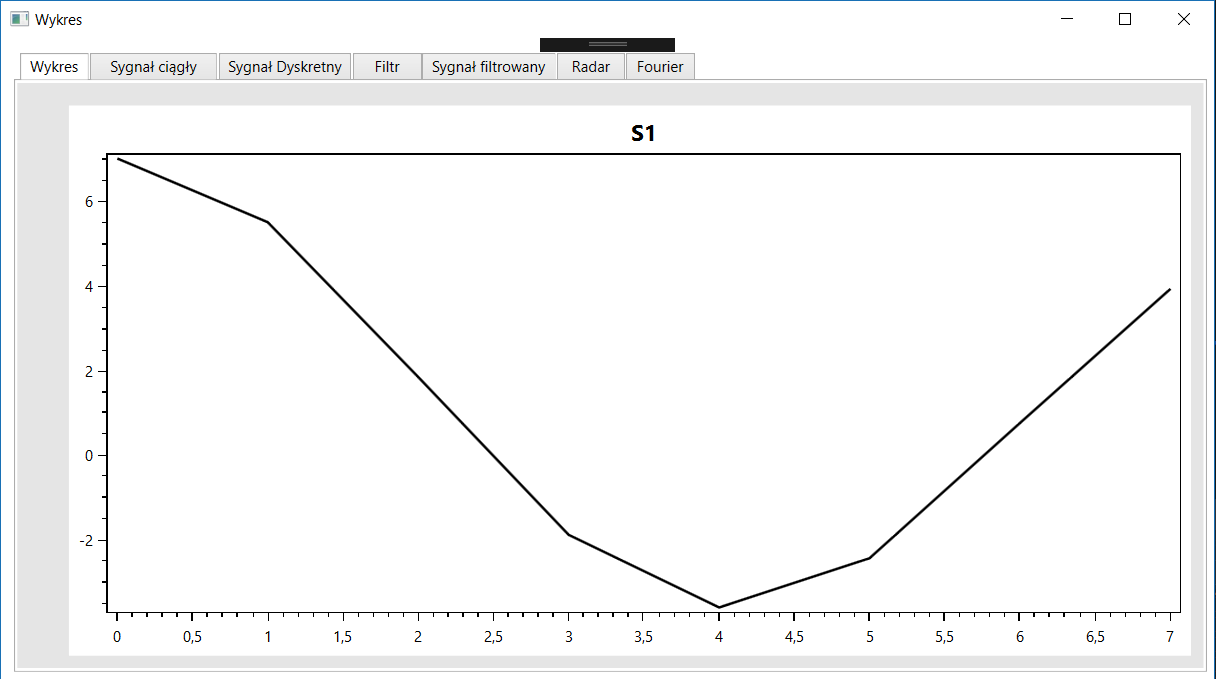
\includegraphics[width=12.3cm]{s13.PNG}
 \vspace{-0.3cm}
 \caption{Wykres funkcji}
 \label{sin}
\end{figure}


\item [Sygnał 2:] 
\subitem [ n:] 6
\begin{figure}[h!]
 \centering
 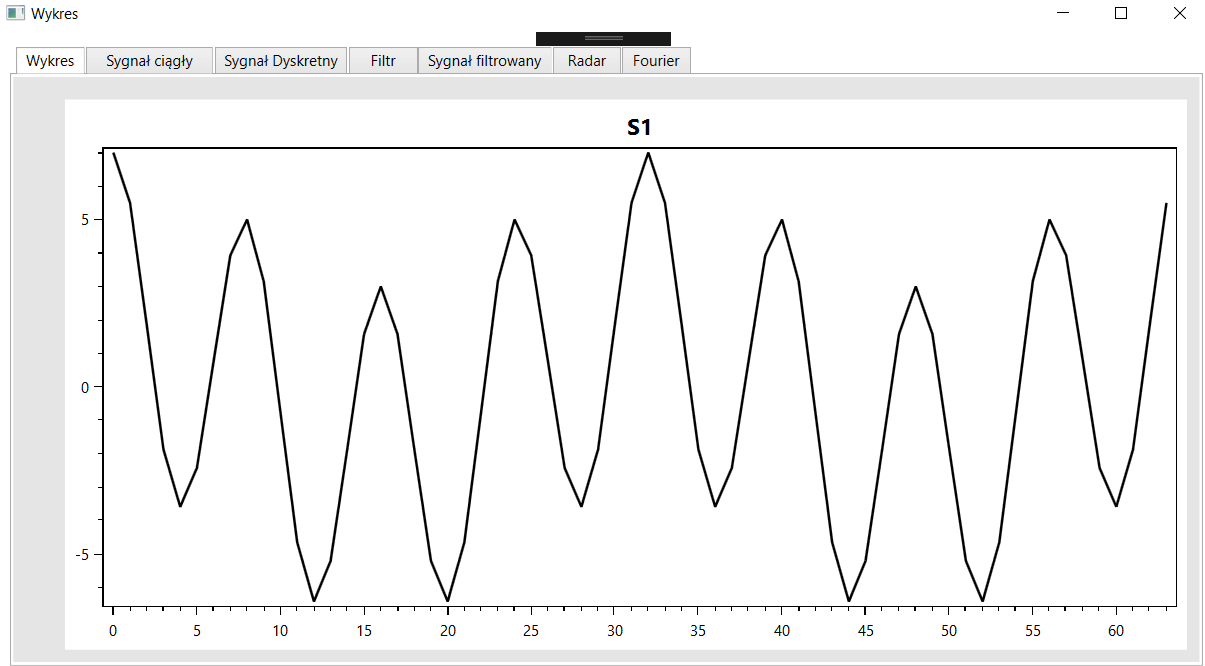
\includegraphics[width=12.3cm]{s16.PNG}
 \vspace{-0.3cm}
 \caption{Wykres funkcji}
 \label{sin}
\end{figure}
\newpage
\item [Sygnał 3:] 
\subitem [ n:] 8
\begin{figure}[h!]
 \centering
 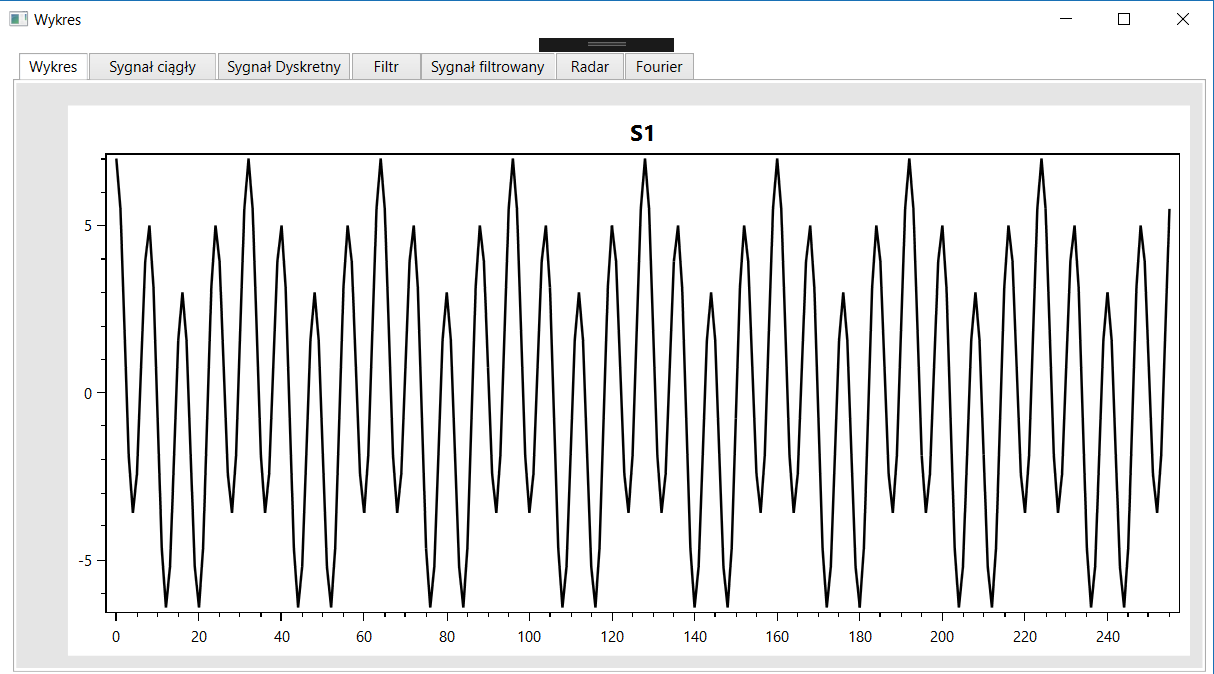
\includegraphics[width=12.3cm]{s18.PNG}
 \vspace{-0.3cm}
 \caption{Wykres funkcji}
 \label{sin}
\end{figure}


\end{labeling}

\subsubsection{Rezultat}

Rezultaty przedstawiają zamieszczone poniżej zrzut ekranu z programu. Czas wykonania oraz wykres transformaciji kosinusowej typu drugiego

 Sygnał 1:
\begin{figure}[h!]
 \centering
 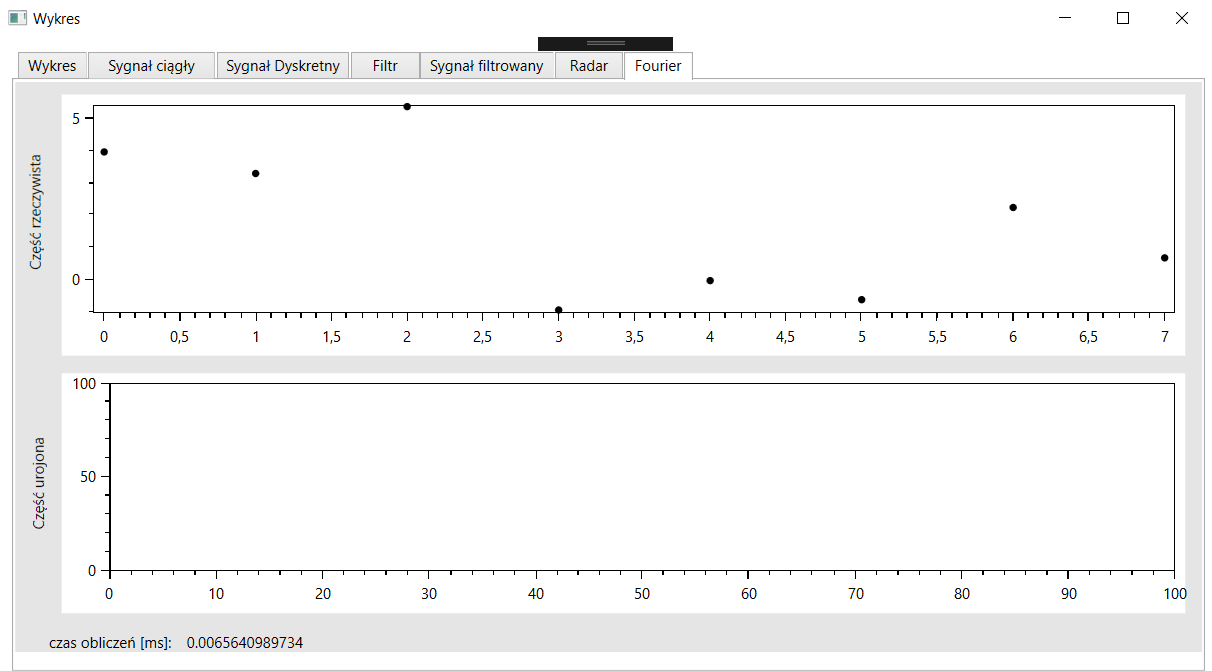
\includegraphics[width=12.3cm]{s13FCT2.PNG}
 \vspace{-0.3cm}
 \caption{Wykres FCT II dla sygnału 1}
 \label{Wykres dla wyników eksperymentu pierwszego}
\end{figure}

Sygnał 2:
\begin{figure}[h!]
 \centering
 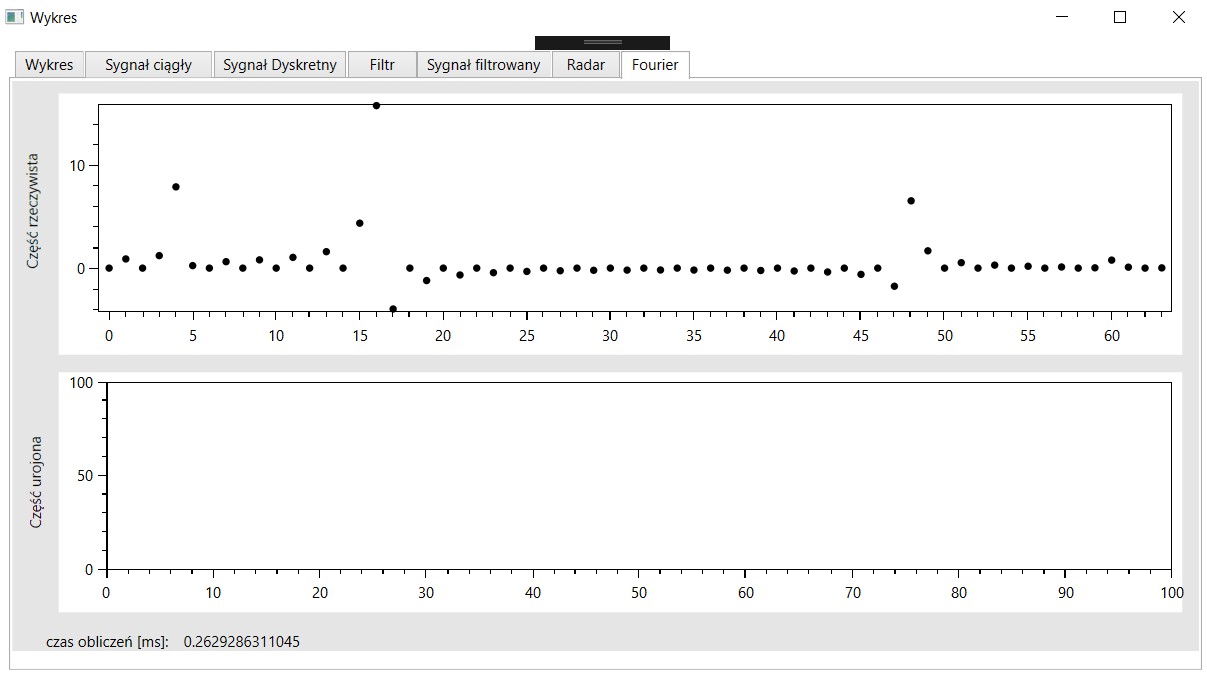
\includegraphics[width=12.3cm]{s16FCT2.PNG}
 \vspace{-0.3cm}
 \caption{Wykres FCT II dla sygnału 2}
 \label{Wykres dla wyników eksperymentu pierwszego}
\end{figure}

\newpage
Sygnał 3:
\begin{figure}[h!]
 \centering
 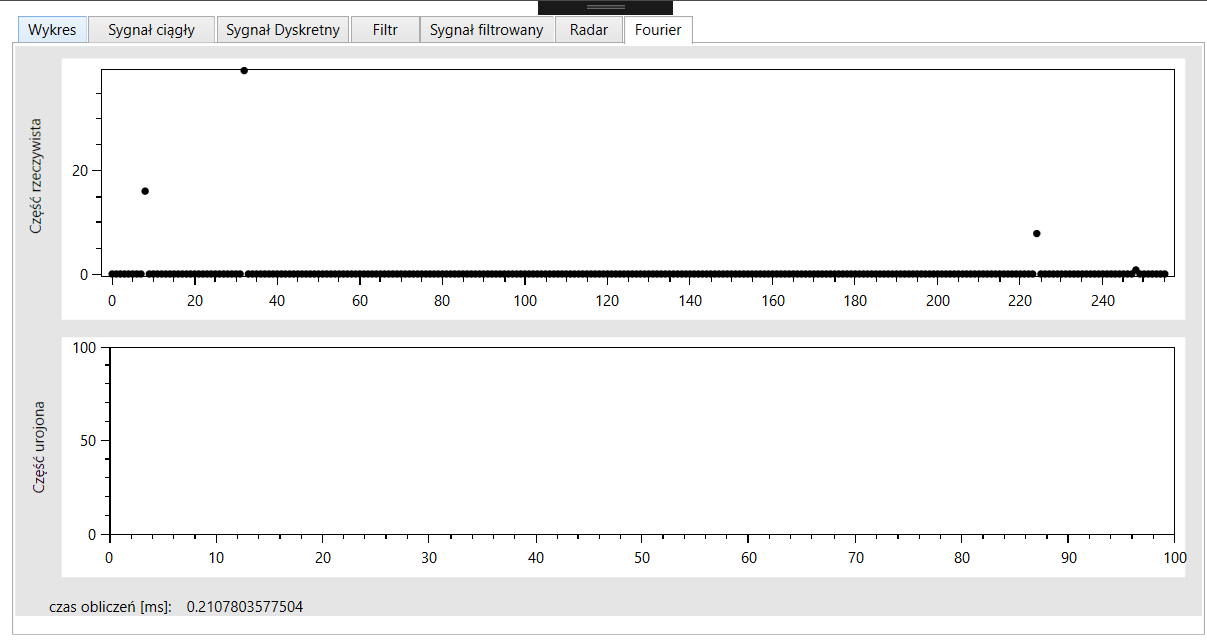
\includegraphics[width=12.3cm]{s18FCT2.PNG}
 \vspace{-0.3cm}
 \caption{Wykres FCT II dla sygnału 3}
 \label{Wykres dla wyników eksperymentu pierwszego}
\end{figure}


%%%%%%%%%%%%%%%%%%%%%%%%%%%%%%%%%%%%%%%%%%%%%%%%%%%%%%%%%%%%%%%%%%%%%%%%%%%%%%%%%%%%%%%%%%%%%%%%%%%%%%%%%%%%%%%%%
% PODROZDZIA PT. EKSPERYMENT NR 5
%%%%%%%%%%%%%%%%%%%%%%%%%%%%%%%%%%%%%%%%%%%%%%%%%%%%%%%%%%%%%%%%%%%%%%%%%%%%%%%%%%%%%%%%%%%%%%%%%%%%%%%%%%%%%%%%%
\section{Podsumowanie}
W poniższych tabelach zostały zebrane czasy wykonania i metody dla każego z naszych sygnałów.
Sygnał 1:
\begin{tabular}{c r @{,} l}
Metoda &
\multicolumn{2}{c}{Czas}\\ \hline
$DFT$ & 0&56825 \\
$FFT$ & 0&00656 \\
$DCT II$ & 0&00514 \\
$FCT II$ & 0&00911 \\
\end{tabular}

Sygnał 2:
\begin{tabular}{c r @{,} l}
Metoda &
\multicolumn{2}{c}{Czas}\\ \hline
$DFT$ & 0&056852 \\
$FFT$ & 0&045219 \\
$DCT II$ & 0&33659 \\
$FCT II$ & 0&05872 \\
\end{tabular}

Sygnał 3:
\begin{tabular}{c r @{,} l}
Metoda &
\multicolumn{2}{c}{Czas}\\ \hline
$DFT$ & 0&31398 \\
$FFT$ & 0&26199 \\
$DCT II$ & 5&41027 \\
$FCT II$ & 0&21078 \\
\end{tabular}


%%%%%%%%%%%%%%%%%%%%%%%%%%%%%%%%%%%%%%%%%%%%%%%%%%%%%%%%%%%%%%%%%%%%%%%%%%%
% PODROZDZIA PT. WNIOSKI
%%%%%%%%%%%%%%%%%%%%%%%%%%%%%%%%%%%%%%%%%%%%%%%%%%%%%%%%%%%%%%%%%%%%%%%%%%%

\section{Wnioski}
Pary algorytmów DFT i FFT oraz DCT II i FCT II dają te same wyniki. Różnią się kosztem obliczeniowym i czasem wykonania. W naszym programie zgodnie z założeniami FFT okazało się szybsze niż DFT, oraz FCT II, w którym został użyty algorytm FFT ma lepsze wyniki niz DCT II.

%%%%%%%%%%%%%%%%%%%%%%%%%%%%%%%%%%%%%%%%%%%%%%%%%%%%%%%%%%%%%%%%%%%%%%%%%%%
% PODROZDZIA PT. ZALACZNIKI
%%%%%%%%%%%%%%%%%%%%%%%%%%%%%%%%%%%%%%%%%%%%%%%%%%%%%%%%%%%%%%%%%%%%%%%%%%%
\begin{thebibliography}{0}
 \bibitem{l2short} FTIMS Politechnika Łódzka.
    \textsl{Zadanie nr 4 - Przekształcenie Fouriera, Walsha-Hadamarda, kosinusowe i falkowe, szybkie algorytmy}, Wikamp.
\end{thebibliography}

\end{document}